% Chapter 4: Experimental Results
% This chapter reports the numerical results from the causal inference and
% predictive frameworks developed in Chapter 3.

This chapter reports the empirical results obtained from the methodology developed in Chapter 3. It first presents estimation diagnostics and then reports the main treatment effect estimates, heterogeneous-effect patterns, robustness checks, and predictive results.

\section{Estimation Diagnostics}
\label{sec:sample-description}

Before estimation, multicollinearity among the three treatment variables was assessed using Variance Inflation Factors (VIF). All three variables have very low VIF values. Since \cite{obrien2007} warns against rigid threshold rules, these values are interpreted as evidence of limited collinearity in this model. Table~\ref{tab:vif-results} shows that \textit{Hype Intensity}, \textit{Urgency Index}, and \textit{Instruction Density} all have VIF values below 1.2.

\begin{table}[htbp]
\centering
\caption{Variance Inflation Factors for Treatment Variables}
\label{tab:vif-results}
\begin{tabular}{|l|r|}
\toprule
\multicolumn{1}{|c|}{\textbf{Treatment Variable}} & \multicolumn{1}{c|}{\textbf{VIF}} \\
\midrule
\textit{Hype Intensity} & 1.189 \\
\textit{Urgency Index} & 1.157 \\
\textit{Instruction Density} & 1.126 \\
\bottomrule
\end{tabular}
\datasetsource
\end{table}

The DML estimator relies on nuisance models to residualize both the outcome and the treatment. The treatment model has a mean cross-validated $R^2$ of $-0.12$ with a range from $-0.29$ to $-0.06$, which indicates low predictive power of the observed confounders for treatment intensity in this sample rather than a close fit of the treatment model. The outcome model has a mean cross-validated $R^2$ of 0.39 for the \textit{10-Minute Logarithmic Return}, which suggests moderate predictive power of the confounders for the outcome and supports the residualization step in the DML procedure. By residualizing the treatment as well, the estimator ensures that the resulting causal coefficients remain orthogonal to observed market factors, protecting the validity of the effect even when treatment intensity is difficult to predict. Taken together, these diagnostics indicate that the model setup is estimable and that the residualization step captures useful outcome variation.

\section{Stratified Average Treatment Effects}
\label{sec:ate-results}

Table~\ref{tab:stratified-ate-results} reports the stratified Average Treatment Effect estimates for each treatment variable across the \textit{Market Capitalization} strata defined in Section~\ref{sec:stratified-estimation}. These estimates compare treatment effects across market-cap groups.

\begin{table}[htbp]
\centering
\caption{Stratified Average Treatment Effects by \textit{Market Capitalization}}
\label{tab:stratified-ate-results}
\small
\begin{tabular}{|l|l|r|r|r|}
\toprule
\multicolumn{1}{|c|}{\textbf{Stratum}} & \multicolumn{1}{c|}{\textbf{Treatment}} & \multicolumn{1}{c|}{\textbf{N}} & \multicolumn{1}{c|}{\textbf{Coefficient}} & \multicolumn{1}{c|}{\textbf{p-value (\%)}} \\
\midrule
\multicolumn{5}{|l|}{\textit{Micro ($<$10M USD)}} \\
 & \textit{Hype Intensity} & 289 & 0.0034 & 22.0 \\
 & \textit{Urgency Index} & 289 & $-$0.0104 & 36.0 \\
 & \textit{Instruction Density} & 289 & 0.0002 & 18.0 \\
\midrule
\multicolumn{5}{|l|}{\textit{Small (10M USD--100M USD)}} \\
 & \textit{Hype Intensity} & 1,182 & 0.0028 & 6.0 \\
 & \textit{Urgency Index} & 1,182 & 0.0301$^{***}$ & $<$0.1 \\
 & \textit{Instruction Density} & 1,182 & 0.0002 & 8.2 \\
\midrule
\multicolumn{5}{|l|}{\textit{Mid (100M USD--1B USD)}} \\
 & \textit{Hype Intensity} & 967 & $-$0.0007 & 10.0 \\
 & \textit{Urgency Index} & 967 & $-$0.0081$^{*}$ & 1.4 \\
 & \textit{Instruction Density} & 967 & 0.0001 & 8.0 \\
\midrule
\multicolumn{5}{|l|}{\textit{Large ($>$1B USD)}} \\
 & \textit{Hype Intensity} & 479 & $-$0.0004$^{**}$ & 0.8 \\
 & \textit{Urgency Index} & 479 & $-$0.0024$^{*}$ & 1.6 \\
 & \textit{Instruction Density} & 479 & $-$0.0001$^{*}$ & 1.0 \\
\bottomrule
\end{tabular}

\source{Own elaboration based on the thesis dataset. Winsorized outcomes at 1\% and 99\%. Statistical significance: $^{***}p<0.1\%$, $^{**}p<1\%$, $^{*}p<5\%$.}
\end{table}

The stratified estimates show a market-cap gradient in treatment effects, especially for \textit{Urgency Index}. The clearest positive coefficient appears in the small-cap stratum, where the \textit{Urgency Index} estimate is 0.0301 (p $<$ 0.1\%). The corresponding estimate turns negative in the mid-cap stratum ($-$0.0081, p = 1.4\%) and remains negative in the large-cap stratum ($-$0.0024, p = 1.6\%).

The micro-cap stratum has no treatment coefficient that reaches conventional significance. This stratum also has the smallest number of observations (N = 289), while the small- and mid-cap strata contain 1,182 and 967 observations, respectively. In the small-cap stratum, \textit{Hype Intensity} and \textit{Instruction Density} show smaller positive coefficients than \textit{Urgency Index}, while all three treatment variables have negative significant estimates in the large-cap stratum.

\section{Heterogeneous Treatment Effects}
\label{sec:hte-results}

The Causal Forest results show how treatment effects vary continuously with \textit{Market Capitalization}. Following Section~\ref{sec:causal-forests}, the analysis uses the market-cap measure as the effect modifier. Table~\ref{tab:cate-summary} reports the distribution of Conditional Average Treatment Effects (CATEs) across the sample for each treatment variable.

\begin{table}[htbp]
\centering
\caption{CATE Summary Statistics by Treatment}
\label{tab:cate-summary}
\begin{tabular}{|l|r|r|r|r|}
\toprule
\multicolumn{1}{|c|}{\textbf{Treatment}} & \multicolumn{1}{c|}{\textbf{Mean}} & \multicolumn{1}{c|}{\textbf{Std. Dev.}} & \multicolumn{1}{c|}{\textbf{Min}} & \multicolumn{1}{c|}{\textbf{Max}} \\
\midrule
\textit{Hype Intensity} & 0.0015 & 0.0028 & $-$0.009 & 0.016 \\
\textit{Urgency Index} & 0.0008 & 0.0258 & $-$0.057 & 0.131 \\
\textit{Instruction Density} & 0.0001 & 0.0002 & $-$0.001 & 0.001 \\
\bottomrule
\end{tabular}
\datasetsource
\end{table}

Figure~\ref{fig:hte-market-cap} shows the relationship between \textit{Market Capitalization} and the heterogeneous effect of \textit{Urgency Index}. Each point represents an event-level CATE estimate. The smoothed trend indicates that the strongest positive effects appear in the lower market-cap range (about 7 million USD to 40 million USD), while effects decline and turn negative for larger assets.

\begin{figure}[htbp]
\centering
\caption[Heterogeneous treatment effect of \textit{Urgency Index} by \textit{Market Capitalization}]{Heterogeneous treatment effect of \textit{Urgency Index} by \textit{Market Capitalization} (event-level CATE estimates with locally smoothed trend).}
\label{fig:hte-market-cap}
\begin{tikzpicture}
    \node[inner sep=0] (img) {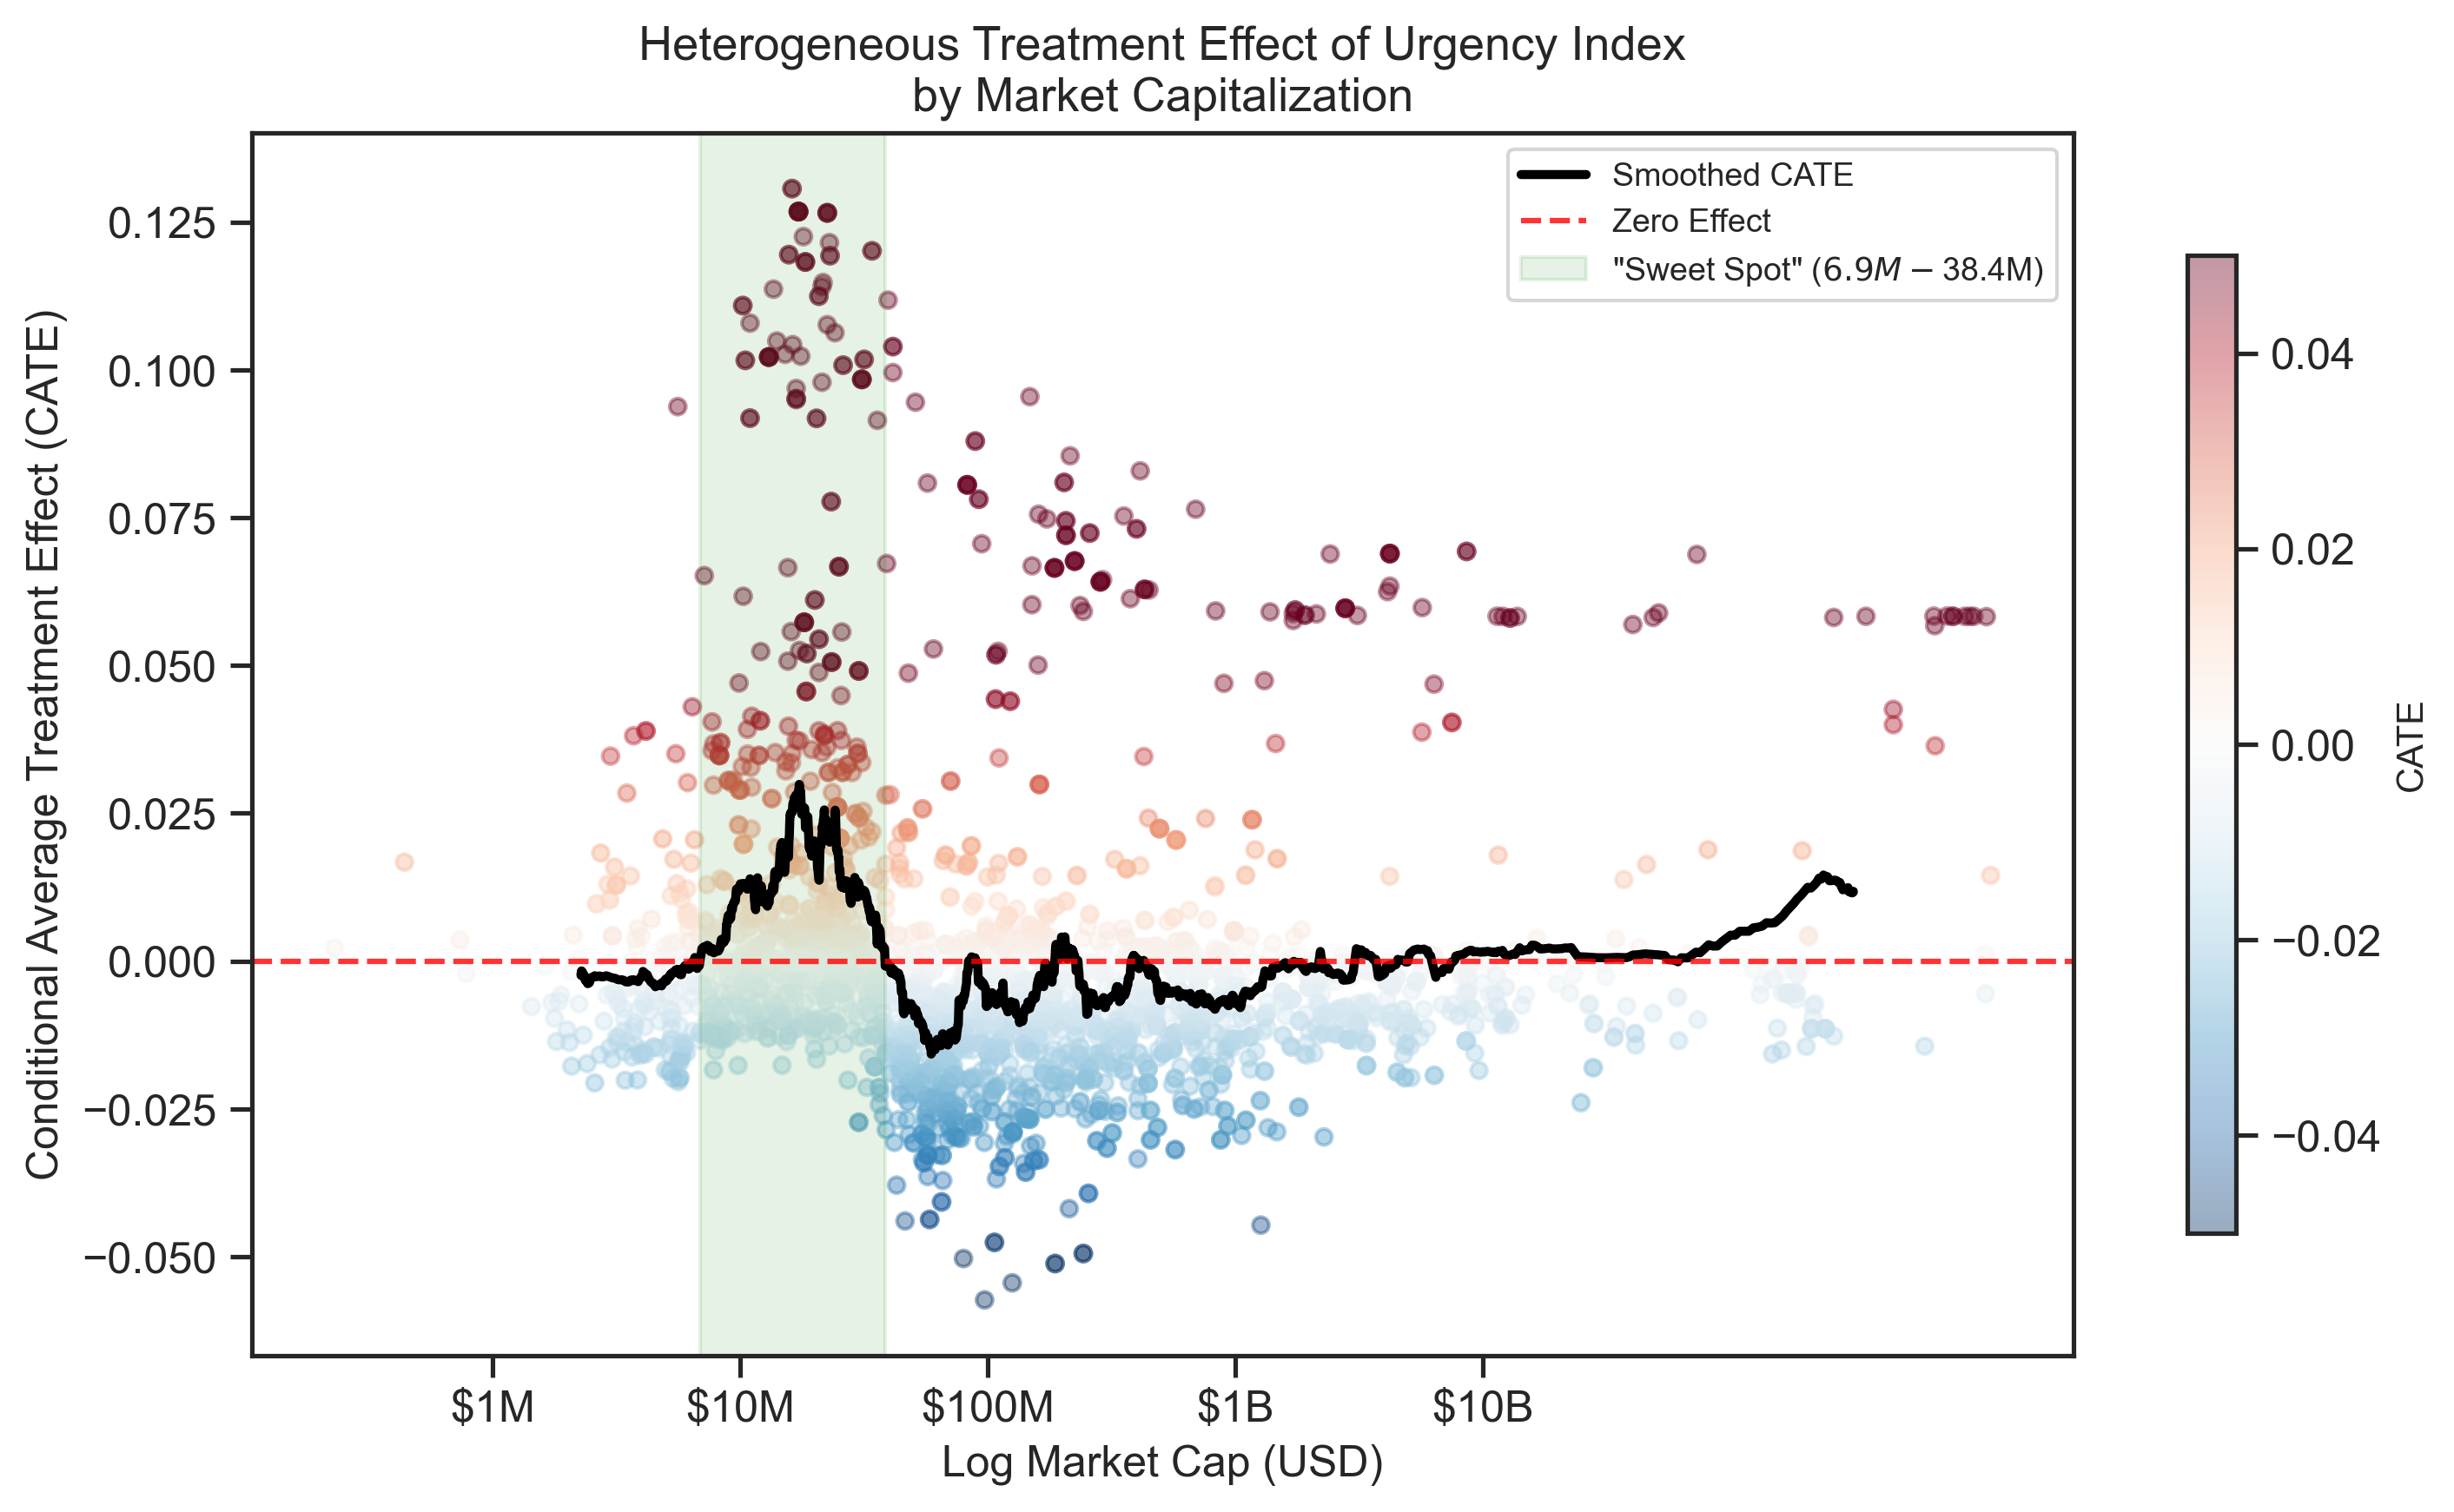
\includegraphics[width=\textwidth,trim=0 0 0 12.5mm,clip]{figures/ch4/hte_market_cap_urgency_index.png}};
    \draw[line width=0.45pt,black,line cap=rect] ([yshift=-0.25pt,xshift=0.102\textwidth]img.north west) -- ([yshift=-0.25pt,xshift=-0.158\textwidth]img.north east);
\end{tikzpicture}
\source{Own elaboration based on the thesis dataset. Note: \textdollar{} denotes USD; M denotes million; B denotes billion.}
\end{figure}

This continuous pattern is consistent with the stratified estimates, with higher positive CATE values concentrated in the lower market-cap range.

\section{Sensitivity Analysis}
\label{sec:robustness}

These results assess whether the statistically significant estimates reported above are sensitive to unmeasured confounding. Table~\ref{tab:evalue-results} reports approximate E-value sensitivity diagnostics based on \cite{vanderweele2017sensitivity}.

\begin{table}[htbp]
\centering
\caption{E-Value Sensitivity Analysis for Significant Effects}
\label{tab:evalue-results}
\begin{tabular}{|l|l|r|r|}
\toprule
\multicolumn{1}{|c|}{\textbf{Stratum}} & \multicolumn{1}{c|}{\textbf{Treatment}} & \multicolumn{1}{c|}{\textbf{E-value}} & \multicolumn{1}{c|}{\textbf{E-value (CI)}} \\
\midrule
Small (10M USD--100M USD) & \textit{Urgency Index} & 2.20 & 1.90 \\
Mid (100M USD--1B USD) & \textit{Urgency Index} & 2.16 & 1.38 \\
Large ($>$1B USD) & \textit{Hype Intensity} & 1.26 & 1.18 \\
Large ($>$1B USD) & \textit{Urgency Index} & 1.95 & 1.41 \\
Large ($>$1B USD) & \textit{Instruction Density} & 1.08 & 1.01 \\
\bottomrule
\end{tabular}
\datasetsource
\end{table}

Approximate E-value diagnostics are reported as sensitivity checks for unmeasured confounding. Higher values suggest that a stronger unmeasured confounder would be needed to explain away the estimate, under the reported calculation. Specifically, the E-value for the small-cap \textit{Urgency Index} effect (2.20) suggests that an unmeasured confounder would need a moderately strong association with both treatment and outcome to fully explain away the estimate. This sensitivity result should be read as an approximate diagnostic rather than definitive proof of robustness.


\section{Predictive Modeling of Pump \textit{Success}}
\label{sec:prediction-results}

This section reports the predictive results for pump \textit{Success}, defined in Chapter~\ref{ch:methodology} as a positive \textit{10-Minute Logarithmic Return}. After testing the candidate tree-based models described in Section~\ref{sec:predictive-modeling}, the XGBoost model was selected as the best performing model and evaluated with the grouped holdout protocol. This unseen-channel evaluation is important because Figure~\ref{fig:channel-returns-distribution} shows that outcomes differ descriptively across channels.

Table~\ref{tab:classification-no-channel} presents the test set performance for this no-channel model.

\begin{table}[htbp]
\centering
\caption{Predictive Performance: No-\textit{Channel ID} XGBoost (Grouped Holdout Test Set)}
\label{tab:classification-no-channel}
\begin{tabular}{|l|c|c|c|c|}
\toprule
\multicolumn{1}{|c|}{\textbf{Metric}} & \multicolumn{1}{c|}{\textbf{Precision}} & \multicolumn{1}{c|}{\textbf{Recall}} & \multicolumn{1}{c|}{\textbf{F1-Score}} & \multicolumn{1}{c|}{\textbf{Support}} \\
\midrule
Fail/Marginal (0) & 0.87 & 0.64 & 0.74 & 437 \\
\textit{Success} ($>$0\%) (1) & 0.69 & 0.89 & 0.78 & 385 \\
\midrule
Macro Avg & 0.78 & 0.77 & 0.76 & 822 \\
\bottomrule
\end{tabular}
\datasetsource
\end{table}

The strictly held-out model reaches a macro F1-score of 0.76. The model achieves 0.89 recall for pump \textit{Success} cases, showing that it identifies many positive outcomes even when observing completely unseen channels.

An additional evaluation was conducted to test whether formally including \textit{Channel ID} could improve predictive performance. That setup did not yield better results across test cases.

\begin{table}[htbp]
\centering
\caption{Decision-Threshold Sensitivity for the No-\textit{Channel ID} XGBoost Model}
\label{tab:threshold-optimization}
\begin{tabular}{|l|c|c|c|c|}
\toprule
\multicolumn{1}{|c|}{\textbf{Threshold}} & \multicolumn{1}{c|}{\textbf{Precision}} & \multicolumn{1}{c|}{\textbf{Recall}} & \multicolumn{1}{c|}{\textbf{F1-Score}} & \multicolumn{1}{c|}{\textbf{Trades}} \\
\midrule
0.50 & 0.686 & 0.891 & 0.775 & 500 \\
0.55 & 0.693 & 0.875 & 0.774 & 486 \\
0.60 & 0.709 & 0.862 & 0.778 & 468 \\
0.65 & 0.723 & 0.834 & 0.774 & 444 \\
0.70 & 0.737 & 0.787 & 0.761 & 411 \\
0.75 & 0.778 & 0.766 & 0.772 & 379 \\
0.80 & 0.791 & 0.720 & 0.754 & 350 \\
0.85 & 0.829 & 0.668 & 0.740 & 310 \\
0.90 & 0.887 & 0.590 & 0.708 & 256 \\
\bottomrule
\end{tabular}
\datasetsource
\end{table}

The threshold results show the expected precision-recall trade-off. Higher thresholds improve precision at the cost of recall and overall trade frequency. Raising the threshold to 0.90 increases precision to 88.7\%, meaning that almost 9 in 10 predicted positive events are positive-return events in the held-out dataset, while retaining 256 predicted events.

To understand which features the model relies on for these predictive results, Figure~\ref{fig:feature-importance-no-channel} presents the top feature importances for the XGBoost model. The leading groups include signal characteristics, weekend timing, asset maturity, short-run relative volume, and market-thinness indicators such as Amihud illiquidity, zero-return ratios, and Roll spread estimates.

\begin{figure}[htbp]
\centering
\caption{Feature importance for predicting pump \textit{Success}. The plot aggregates the relative importance of predictive groups derived from the XGBoost model.}
\label{fig:feature-importance-no-channel}
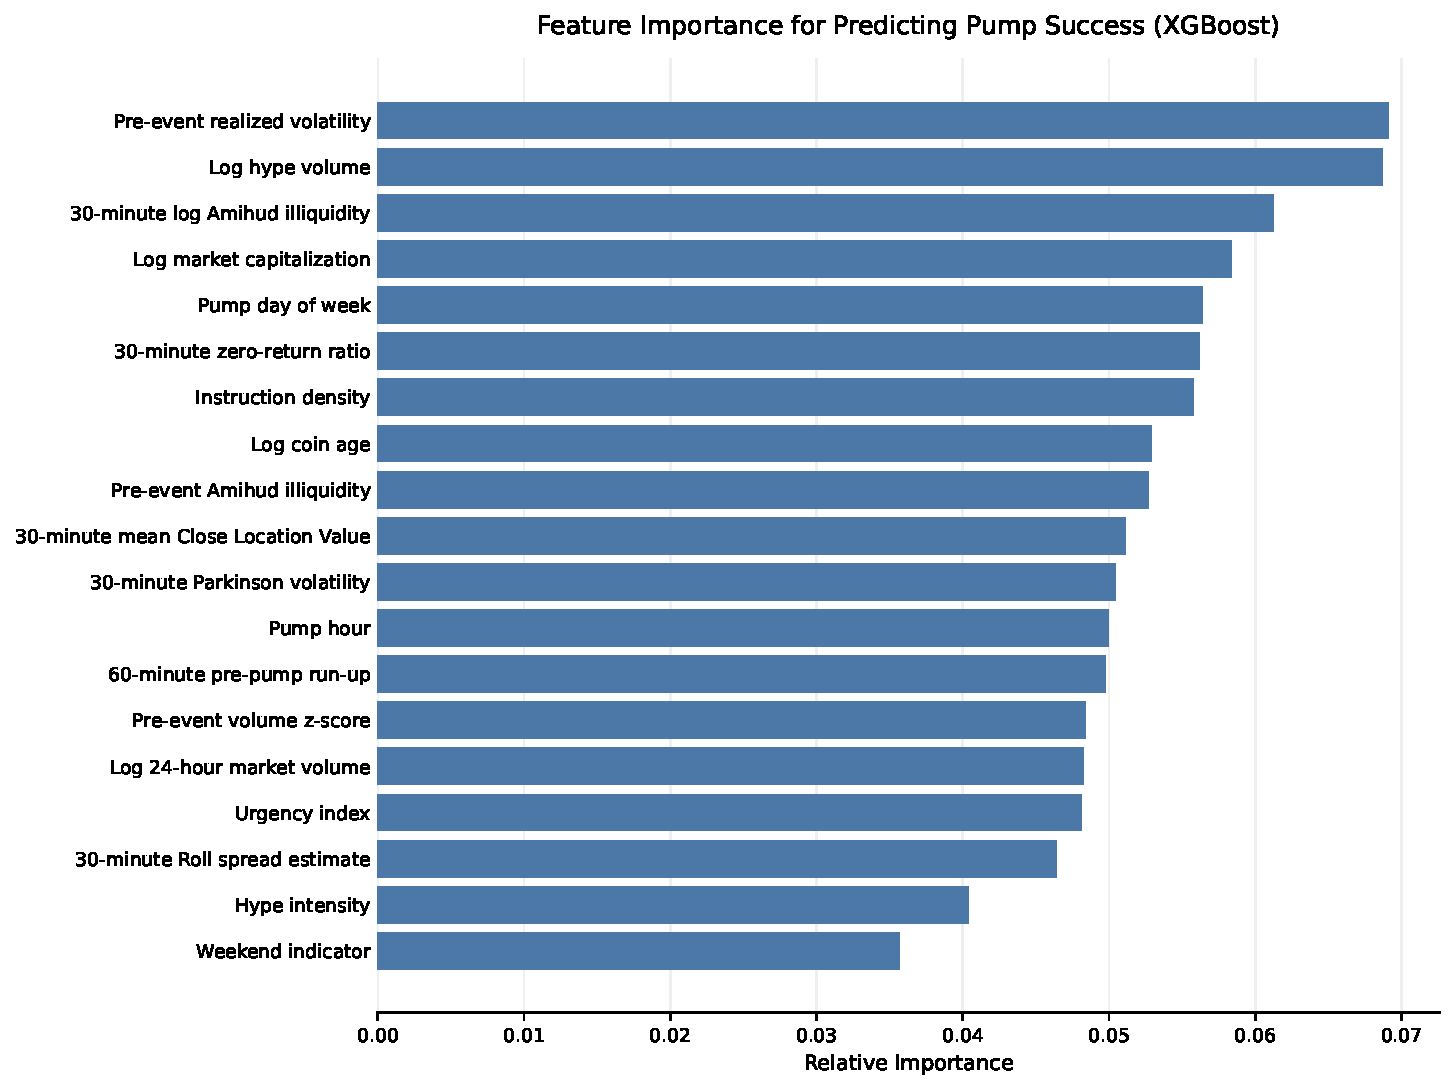
\includegraphics[width=0.85\textwidth,trim=0 0 0 7mm,clip]{figures/ch4/feature_importance_without_channel.pdf}
\datasetsource
\end{figure}
